\documentclass[12pt]{article}

% ============================================================
% IDIOMA Y CODIFICACIÓN
% ============================================================
\usepackage[utf8]{inputenc}
\usepackage[T1]{fontenc}

% ============================================================
% COLOR Y TABLAS CON COLOR
% ============================================================
\usepackage[dvipsnames]{xcolor}
\usepackage{colortbl}

% ============================================================
% MÁRGENES Y GEOMETRÍA
% ============================================================
\usepackage[a4paper, margin=2.5cm]{geometry}

% ============================================================
% ESPACIADO
% ============================================================
\usepackage{setspace}
\setstretch{1.15}
\setlength{\parskip}{0.5em}
\setlength{\parindent}{0pt}

% ============================================================
% TIPOGRAFÍA
% ============================================================
\usepackage{lmodern}

% ============================================================
% FORMATO DE TÍTULOS
% ============================================================
\usepackage{titlesec}

\titleformat{\section}
  {\Large\bfseries}{\thesection.}{0.5em}{}
\titlespacing*{\section}{0pt}{1.5em}{0.8em}

\titleformat{\subsection}
  {\large\bfseries}{\thesubsection.}{0.5em}{}
\titlespacing*{\subsection}{0pt}{1em}{0.5em}

% ============================================================
% MATEMÁTICAS
% ============================================================
\usepackage{amsmath, amssymb, amsfonts}

% ============================================================
% GRÁFICOS Y ÁRBOLES
% ============================================================
\usepackage{graphicx}
\usepackage{float}
\usepackage{tikz}
\usepackage[edges]{forest}
\usetikzlibrary{arrows.meta, trees, shapes.geometric, positioning, calc}

% ============================================================
% TABLAS
% ============================================================
\usepackage{booktabs}
\usepackage{array}
\usepackage{multirow}

% ============================================================
% CÓDIGO FUENTE
% ============================================================
\usepackage{listings}

\definecolor{codebg}{RGB}{248,248,248}
\definecolor{codeframe}{RGB}{200,200,200}
\definecolor{codecomment}{RGB}{106,153,85}
\definecolor{codekeyword}{RGB}{86,156,214}
\definecolor{codestring}{RGB}{206,145,120}
\definecolor{codenumber}{RGB}{181,206,168}

\lstdefinestyle{estilo_base}{
    backgroundcolor=\color{codebg},
    frame=single,
    rulecolor=\color{codeframe},
    basicstyle=\ttfamily\small,
    commentstyle=\color{codecomment}\itshape,
    keywordstyle=\color{codekeyword}\bfseries,
    stringstyle=\color{codestring},
    numberstyle=\tiny\color{codenumber},
    numbers=left, numbersep=8pt,
    breaklines=true, breakatwhitespace=true,
    tabsize=4, showstringspaces=false, captionpos=b,
    literate=
        {á}{{\'a}}1 {é}{{\'e}}1 {í}{{\'i}}1 {ó}{{\'o}}1 {ú}{{\'u}}1
        {Á}{{\'A}}1 {É}{{\'E}}1 {Í}{{\'I}}1 {Ó}{{\'O}}1 {Ú}{{\'U}}1
        {ñ}{{\~n}}1 {Ñ}{{\~N}}1 {ü}{{\"u}}1 {¿}{{?`}}1 {¡}{{!`}}1,
}

% ============================================================
% LISTAS
% ============================================================
\usepackage{enumitem}

% ============================================================
% ENLACES
% ============================================================
\usepackage{hyperref}
\hypersetup{
    colorlinks=true, linkcolor=black,
    urlcolor=blue!60!black, citecolor=black,
    pdftitle={Introducción a las Estructuras de Datos - Trabajo Práctico Integrador},
    pdfauthor={Facundo Luna},
}

% ============================================================
% ENCABEZADO Y PIE DE PÁGINA
% ============================================================
\usepackage{fancyhdr}
\pagestyle{fancy}
\fancyhf{}
\renewcommand{\headrulewidth}{0.4pt}
\renewcommand{\footrulewidth}{0.4pt}
\fancyhead[L]{\small Introducción a las Estructuras de Datos}
\fancyhead[R]{\small Trabajo Práctico Integrador}
\fancyfoot[L]{\small Facundo Luna}
\fancyfoot[R]{\small \thepage}

% ============================================================
% DATOS DEL TRABAJO
% ============================================================
\newcommand{\universidad}{Universidad Católica de Salta}
\newcommand{\carrera}{Licenciatura en Ciencia de Datos}
\newcommand{\materia}{Introducción a las Estructuras de Datos}
\newcommand{\trabajo}{Trabajo Práctico Integrador}
\newcommand{\profesor}{Ing. Carlos Pastrana}
\newcommand{\alumno}{Facundo Luna}
\newcommand{\fecha}{\today}

\newcommand{\logoincluido}{%
    
\includegraphics[width=3.5cm]{../../../assets/ucasal-logo.png}\\[0.5cm]%
}
\newcommand{\logoomitido}{\vspace{1cm}}
\newcommand{\logoportada}{\logoincluido}

% ============================================================
% COMANDOS AUXILIARES
% ============================================================
\newcommand{\solucion}{%
    \vspace{0.8em}\textbf{Solución:}\par\vspace{0.4em}%
}

\newcommand{\volverindice}{%
    \vspace{1em}%
    \begin{flushright}%
        \hyperlink{indice}{\small $\uparrow$ Volver al índice}%
    \end{flushright}%
}

% ============================================================

\begin{document}

% ======================== PORTADA ===========================
\begin{titlepage}
    \centering
    \logoportada
    \rule{\linewidth}{1.5pt}\\[0.4cm]
    {\large\scshape \universidad}\\[0.2cm]
    {\large \carrera}\\[0.1cm]
    \rule{\linewidth}{0.5pt}\\[1.5cm]
    {\Huge\bfseries \trabajo}\\[0.8cm]
    {\LARGE \materia}\\[2cm]
    \begin{tabular}{rl}
        \textbf{Alumno:}   & \alumno   \\[0.3cm]
        \textbf{Profesor:} & \profesor \\[0.3cm]
        \textbf{Fecha:}    & \fecha    \\
    \end{tabular}
    \vfill
    \rule{\linewidth}{1.5pt}
\end{titlepage}

% ======================== ÍNDICE ============================
\newpage
\hypertarget{indice}{}
\tableofcontents
\setcounter{tocdepth}{2}

% ==============================================================
% ACTIVIDAD 1 - GRAFOS
% ==============================================================
\newpage
\section{Análisis de grafo}

\textit{Dado el siguiente grafo:}

\begin{figure}[H]
\centering
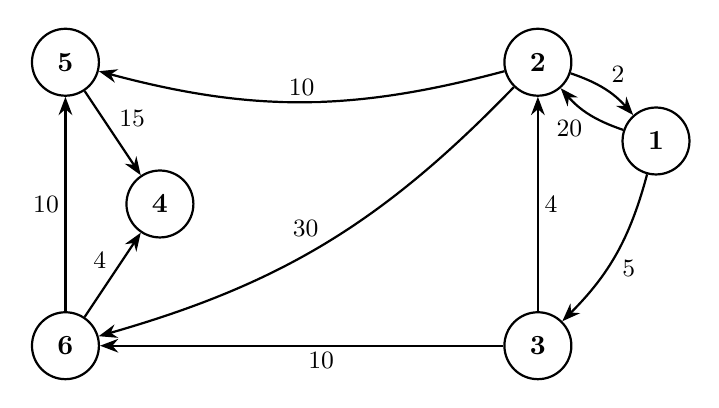
\begin{tikzpicture}[
    every path/.style={thick},
    ->,
    >=Stealth
]
    \tikzset{
        vertice/.style={circle, draw, thick, minimum size=0.85cm, font=\bfseries},
        peso/.style={font=\small, fill=white, inner sep=2pt}
    }

    % Nodos
    \node[vertice] (5) at (0, 0)     {5};
    \node[vertice] (2) at (6, 0)     {2};
    \node[vertice] (1) at (7.5,-1)   {1};
    \node[vertice] (4) at (1.2,-1.8) {4};
    \node[vertice] (6) at (0, -3.6)  {6};
    \node[vertice] (3) at (6, -3.6)  {3};

    % Aristas
    \draw (5) to node[peso, above right]        {15} (4);
    \draw (2) to[bend left=15]  node[peso, above right] {2}  (1);
    \draw (2) to[bend left=15]  node[peso, above left]  {30} (6);
    \draw (2) to[bend left=15]  node[peso, above]       {10} (5);
    \draw (1) to[bend left=15]  node[peso, below left]  {20} (2);
    \draw (1) to[bend left=15]  node[peso, below right] {5}  (3);
    \draw (3) to node[peso, right]              {4}  (2);
    \draw (6) to node[peso, left]               {10} (5);
    \draw (6) to node[peso, above left]         {4}  (4);
    \draw (3) to node[peso, below right]        {10} (6);
\end{tikzpicture}
\caption{Grafo a analizar}
\label{fig:grafo}
\end{figure}

\subsection{Indicar características del grafo}

\textit{a) Indique:}

\begin{itemize}[leftmargin=2cm]
    \item ¿Es un grafo dirigido, no dirigido?
    \item ¿Es conexo?
    \item ¿Es ponderado?
    \item ¿Maximal? ¿Minimal?
\end{itemize}

\solucion

\begin{itemize}[leftmargin=2cm]
    \item \textbf{Dirigido o no dirigido:} Es un grafo \textbf{dirigido},
    ya que cada arista tiene una dirección definida por una flecha.

    \item \textbf{Conexo:} El grafo es \textbf{débilmente conexo}: ignorando
    las direcciones de las aristas, el grafo subyacente es conexo.
    Sin embargo, \textbf{no es fuertemente conexo}, ya que el nodo~4 no posee
    aristas de salida, por lo que no es posible alcanzar ningún otro nodo
    partiendo desde él.

    \item \textbf{Ponderado:} El grafo \textbf{es ponderado}, ya que cada
    arista tiene un peso numérico asociado.

    \item \textbf{Maximal / Minimal:} El vértice $4$ es maximal porque no posee aristas de salida. No existen vértices minimales, ya que todos los nodos tienen al menos una arista de entrada.
\end{itemize}

\subsection{Matriz de adyacencia}

\textit{b) Represente el grafo mediante una matriz de adyacencia.}

\solucion

La matriz de adyacencia $A$ para los nodos $\{1,2,3,4,5,6\}$ es:

\[
A = \begin{pmatrix}
      & 1  & 2  & 3  & 4  & 5  & 6  \\
    1 & 0  & 20 & 5  & 0  & 0  & 0  \\
    2 & 2  & 0  & 0  & 0  & 10 & 30 \\
    3 & 0  & 4  & 0  & 0  & 0  & 10 \\
    4 & 0  & 0  & 0  & 0  & 0  & 0  \\
    5 & 0  & 0  & 0  & 15 & 0  & 0  \\
    6 & 0  & 0  & 0  & 4  & 10 & 0  \\
\end{pmatrix}
\]
donde $A_{ij} = w$ indica que existe una arista dirigida desde el nodo $i$
hacia el nodo $j$ con peso $w$, y $A_{ij} = 0$ indica su ausencia.

\volverindice

% ==============================================================
% ACTIVIDAD 2 - PILAS Y COLAS
% ==============================================================
\newpage
\section{Algoritmo de pasos básicos con pilas y colas}

\textit{Desarrollar un algoritmo de pasos básicos que me permita recorrer una lista y:}

\textit{a) Al encontrarse un elemento par, deberá generar y mostrar una pila; caso
distinto, al encontrarse con un elemento impar, deberá generar y mostrar una cola
resultante conteniendo los números impares.}

\textit{b) Mostrar el promedio de los elementos de la pila P1.}

\solucion

El algoritmo valida primero que todos los elementos sean enteros.
Si hay alguno inválido, informa el error y termina.
De lo contrario, recorre la lista y apila los pares o encola los impares
según corresponda, para luego calcular el promedio de la pila.

\newpage
\begin{lstlisting}[style=estilo_base, language=Java]
import java.util.ArrayDeque;
import java.util.Arrays;
import java.util.Deque;

public class Ejercicio02 {
    public static void main(String[] args) {
        // lista hardcodeada por simplicidad
        Object[] list = { 0, 1, 2, 3, 4, 5, 6, 7, 8, 9 };
        for (Object elemento : list) {
            // no reservo memoria si hay un elemento inválido
            if (!(elemento instanceof Integer)) {
                System.out.println("Error: '" + elemento + "' no es un número entero.");
                return;
            }
        }

        Integer suma = 0;
        // tipo Deque (interfaz) para no acoplar el código a una implementación
        Deque<Integer> pila = new ArrayDeque<>();
        Deque<Integer> cola = new ArrayDeque<>();

        for (Object elemento : list) {
            Integer numero = (Integer) elemento;
            (numero % 2 == 0 ? pila : cola).add(numero);
        }
        System.out.println("item a)");
        System.out.println("Lista original: " + Arrays.toString(list));
        System.out.println("Pila Auxiliar (pares):   " + pila);
        System.out.println("Cola Auxiliar (impares): " + cola);

        for (Integer par : pila) {
            suma += par; // acumulo para luego dividir por el tamaño de la pila
        }
        System.out.println("item b)");
        System.out.println("El Promedio de la Pila Auxiliar es: "
                + (suma / (double) pila.size()));
    }
}
\end{lstlisting}

\newpage
\textbf{Salida --- caso exitoso} (todos los elementos son enteros):

\begin{lstlisting}[style=estilo_base, language={}, numbers=none]
item a)
Lista original: [0, 1, 2, 3, 4, 5, 6, 7, 8, 9]
Pila Auxiliar (pares):   [0, 2, 4, 6, 8]
Cola Auxiliar (impares): [1, 3, 5, 7, 9]
item b)
El Promedio de la Pila Auxiliar es: 4.0
\end{lstlisting}

\textbf{Salida --- caso de error} (la lista contiene un elemento no entero,
p.\,ej.\ \texttt{"hola"} en la posición 2):

\begin{lstlisting}[style=estilo_base, language={}, numbers=none]
Error: 'hola' no es un número entero.
\end{lstlisting}

\volverindice

% ==============================================================
% ACTIVIDAD 3 - ÁRBOLES
% ==============================================================
\newpage
\section{Análisis de árbol}

\textit{Dado el siguiente árbol:}

\begin{figure}[H]
\centering
\begin{forest}
  for tree={
    draw, circle,
    minimum size=0.8cm,
    inner sep=2pt,
    s sep=1cm,
    l sep=0.8cm,
  }
  [8
    [3
      [1]
      [6
        [4]
        [7]
      ]
    ]
    [10
      [,phantom]
      [14
        [13]
        [,phantom]
      ]
    ]
  ]
\end{forest}
\caption{Árbol binario a analizar}
\label{fig:arbol}
\end{figure}

\subsection{Características del árbol}

\textit{a) Indicar:}

\begin{itemize}[leftmargin=2cm]
    \item ¿Qué tipo de árbol es? ¿Es completo?
    \item ¿Altura?
    \item ¿Se encuentra balanceado? Fundamente
\end{itemize}

\solucion

\begin{itemize}[leftmargin=2cm]
    \item \textbf{Tipo de árbol:} Es un \textbf{árbol binario de búsqueda (ABB)}.
    \textbf{No es completo}, ya que el nodo~10 no tiene hijo izquierdo,
    lo que rompe el requisito de que los nodos del último nivel estén
    alineados a la izquierda.

    \item \textbf{Altura:} Considerando la raíz con altura~1, el árbol
    tiene \textbf{altura~4}.

    \item \textbf{Balanceo:} El árbol \textbf{no está balanceado}.
    Para determinarlo se calcula el Factor de Balance (FB) de cada nodo,
    definido como:
    \[
        FB(n) = \text{altura\_subárbol\_izquierdo}(n) -
                \text{altura\_subárbol\_derecho}(n)
    \]

    \newpage
    Los factores de balance obtenidos son:
    \begin{center}
    \begin{tabular}{cc}
        \toprule
        \textbf{Nodo} & \textbf{FB} \\
        \midrule
        1  &  0 \\
        4  &  0 \\
        7  &  0 \\
        13 &  0 \\
        6  &  0 \\
        14 & $-1$ \\
        3  & $-1$ \\
        10 & $-2$ \\
        8  &  0 \\
        \bottomrule
    \end{tabular}
    \end{center}
    El nodo~10 tiene $FB = -2$, valor fuera del rango $[-1, 1]$
    exigido por un árbol AVL. Por lo tanto, el árbol se considera
    \textbf{desbalanceado}.
\end{itemize}

\subsection{Recorridos del árbol}

\textit{b) Generar los recorridos ``pre order'', ``in order'', ``post order'' del árbol dado.}

\solucion

\begin{itemize}[leftmargin=2cm]
    \item \textbf{In-order} (izquierda $\to$ raíz $\to$ derecha):
    \[
        1,\ 3,\ 4,\ 6,\ 7,\ 8,\ 10,\ 13,\ 14
    \]

    \item \textbf{Pre-order} (raíz $\to$ izquierda $\to$ derecha):
    \[
        8,\ 3,\ 1,\ 6,\ 4,\ 7,\ 10,\ 14,\ 13
    \]

    \item \textbf{Post-order} (izquierda $\to$ derecha $\to$ raíz):
    \[
        1,\ 4,\ 7,\ 6,\ 3,\ 13,\ 14,\ 10,\ 8
    \]
\end{itemize}

\volverindice

% ==============================================================
% ACTIVIDAD 4 - HASH
% ==============================================================
\newpage
\section{Método hash de división con $m = 50$}

\textit{Por el método hash de división con $m=50$, obtener los valores hash de los
siguientes conjuntos de claves: `Ariel', `Luis', `Gonzalo', `Federico', `Roberto', `Carlos'.}

\solucion

Para cada clave se suman los valores ASCII de sus caracteres y se aplica
el módulo $m = 50$. La tabla siguiente detalla el cálculo completo.

\begin{center}
\begin{tabular}{llcc}
\toprule
\textbf{Clave} & \textbf{Suma de valores ASCII} & \textbf{Suma} & $h(k)$ \\
\midrule
Ariel    & $65+114+105+101+108$ & $493$ & $493 \bmod 50 = \mathbf{43}$ \\
Luis     & $76+117+105+115$     & $413$ & $413 \bmod 50 = \mathbf{13}$ \\
Gonzalo  & $71+111+110+122+97+108+111$ & $730$ & $730 \bmod 50 = \mathbf{30}$ \\
Federico & $70+101+100+101+114+105+99+111$ & $801$ & $801 \bmod 50 = \mathbf{1}$  \\
Roberto  & $82+111+98+101+114+116+111$ & $733$ & $733 \bmod 50 = \mathbf{33}$ \\
Carlos   & $67+97+114+108+111+115$ & $612$ & $612 \bmod 50 = \mathbf{12}$ \\
\bottomrule
\end{tabular}
\end{center}

\vspace{0.5em}
No se presentan colisiones entre las claves dadas: los seis valores hash
obtenidos ($43, 13, 30, 1, 33, 12$) son todos distintos.

\volverindice
\end{document}